\documentclass[LaTeX2e,10pt]{beamer}
\usefonttheme{professionalfonts}
\usepackage{siunitx}
%\usepackage{wrapfig}
\usepackage{newtxtext,newtxmath}
\usepackage{bm}
\usepackage{hyperref}
\usepackage{graphicx}
\usepackage{subcaption}
\usepackage{verbatim}  % Needed for the "comment" environment to make LaTeX comments
\usepackage{amsmath}
\usepackage{caption}
\captionsetup{labelformat=empty,labelsep=none}
\setbeamertemplate{caption}{\insertcaption}
\captionsetup[figure]{labelformat=empty} %% to remove the figure from Caption.
\usepackage{tikz} %% For making boxes colored
\usepackage{verbatim}
\usetikzlibrary{arrows,shapes}
\usepackage{xcolor}
\usepackage{graphicx}
\usepackage{psfrag}
\usepackage{epstopdf}
\usepackage{hyperref}
\usepackage{bookmark}
%\usepackage{lmodern}
%\usepackage{subfig}   % For subfigure
\usepackage{array}
\definecolor{sotonWhite}{rgb}{1 1 1} % white
\definecolor{sotonMB}{rgb}{0 0.3594 0.5156} % soton marine blue (7469)
\definecolor{sotonCB}{rgb}{0.1 0.6844 0.7703} % soton cyan blue (3145)
\definecolor{sotonLB}{rgb}{0 0.5938 0.7617} % soton light blue (313)
\definecolor{sotonDG}{rgb}{0.3164 0.3828 0.4336} % soton dark grey (7545)
\definecolor{sotonGR}{rgb}{0.6367 0.5653 0.4180} % soton green (5777)
\definecolor{sotonME}{rgb}{0.7305 0.7305 0.7305} % soton metal (877)
\definecolor{sotonLG}{rgb}{0.6406 0.6797 0.7070} % soton light grey (7543)

\definecolor{sotonyel}{rgb}{.99999 .70196 .00000} % soton yellow
\definecolor{sotonora}{rgb}{.99608 .24314 .07843} % soton orange
\definecolor{sotonred}{rgb}{.94118 .05882 .17255} % soton red
\definecolor{sotonrus}{rgb}{.67059 .07059 .06275} % soton russet
\definecolor{sotonbrn}{rgb}{.54118 .25490 .16863} % soton brown
\definecolor{sotonpnk}{rgb}{.88627 .41176 .62353} % soton pink
\definecolor{sotonppl}{rgb}{.32549 .12157 .26667} % soton purple

\setbeamertemplate{background canvas}[vertical shading][top=sotonWhite,bottom=sotonWhite]
\setbeamercolor{background canvas}{bg=white}
\setbeamercolor{button border}{bg=sotonWhite, fg=sotonWhite}
\setbeamercolor{button}{bg=sotonWhite, fg=sotonWhite}

\setbeamercolor{title page}{fg=black}

\setbeamercolor{block title}{fg=sotonMB}
\setbeamercolor{frametitle}{fg=sotonMB}
\setbeamercolor{framesubtitle}{fg=sotonMB}
\setbeamercolor{alerted text}{fg=sotonMB}
\setbeamercolor{normal text}{fg=darkgray}
\setbeamercolor{titlelike}{fg=sotonMB}
\setbeamercolor{author}{fg=darkgray}
\setbeamercolor{date}{fg=darkgray}
\setbeamercolor{item}{fg=darkgray}
\setbeamercolor{caption name}{fg=darkgray}
\setbeamercolor{footline text}{fg=darkgray}

\newcommand{\putlogo}{\includegraphics[width=3.5cm]{Logos/SotonLogo.eps}} % for UoS

\newcommand{\footline}{\color{sotonMB}\rule{\textwidth}{1pt}}

% ---------- FURTHER DEFINITIONS --------------
\setlength{\unitlength}{1cm}
\graphicspath{{./Graphics/}}
% --------------- END -------------------------

\begin{document}
\setbeamertemplate{headline}{
	%\vspace{6pt}\hspace{10pt}\putlogoUnit\hfill\putlogo\hspace{3.5mm} % logo on the right
	\vspace{6pt}\hspace{10pt}\hfill\putlogo\hspace{3.5mm} % logo on the right
}
\begin{frame}
\center
\huge Linear Vibration Energy Harvesting\\[1em]
\normalsize \href{http://www.ecs.soton.ac.uk/people/bz4c16}{Dr. Bahareh Zaghari}\\[1em]\footnotesize Smart Electronic Materials and Systems Research Group \\ Electronics and Computer Science\\ University of Southampton, UK\\[1em]bahareh.zaghari@soton.ac.uk\\[3em]NiPS Summer School \\ July 17-20, 2018 \\ Perugia, Italy\\[2em]These slides are available on GitHub at https://tinyurl.com/y9uwtz3q.
\end{frame}
\addtocounter{framenumber}{-1} % Do not count the title frame!

\setbeamertemplate{headline}{
%	\vskip25pt % horizontal line
%	\vskip-21pt\hspace{2pt}\hfill\hspace{3.5mm} % logo on the right
}

\setbeamertemplate{footline}{
	\vskip-10pt\footline\\ % horizontal line
	\vskip2pt
	\makebox[123mm]{\hspace{7.5mm}
	\insertshorttitle
	\hfill \insertframenumber}
	\vskip4pt
}
%%%%%%%%%%%%%%%%%%%%%%%%%%%%%%%%%%%%%%%%%%%%%%%%%%%%%%%%%%%%%%%%%%%%%%%%%%%%%%%%%%%%%%%%%%%%%%%%
\tikzstyle{every picture}+=[remember picture]
\everymath{\displaystyle}
%%%%%%%%%%%%%%%%%%%%%%%%%%%%%%%%%%%%%%%%%%%%%%%%%%%%%%%%%%%%%%%%%%%%%%%%%%%%%%%%%%%%%%%%%%%%%%%%
\begin{frame}{Energy harvesting components}
\begin{figure}
	\centering
	\includegraphics[width=\linewidth]{Images/energyHarvestingComponents.eps}
	\caption{}
\end{figure}
\vskip-20pt
Relevant references
\scriptsize
\begin{itemize}
	\item R. S. Langley, \href{https://www.sciencedirect.com/science/article/pii/S0022460X13007906}{A general mass law for broadband energy harvesting}
	\item S. Roundy, \href{http://journals.sagepub.com/doi/abs/10.1177/1045389X05054042}{On the Effectiveness of Vibration-based Energy Harvesting}
	\item K. Nakano et al., \href{http://iopscience.iop.org/article/10.1088/0964-1726/16/4/002/meta}{A unified approach to optimal conditions of power harvesting using electromagnetic and piezoelectric transducers}
	\item C. Cepnik et al., \href{http://www.mdpi.com/2072-666X/4/3/286}{Approaches for a Fair Comparison and Benchmarking of Electromagnetic Vibration Energy Harvesters}
\end{itemize}
\end{frame}
%%%%%%%%%%%%%%%%%%%%%%%%%%%%%%%%%%%%%%%%%%%%%%%%%%%%%%%%%%%%%%%%%%%%%%%%%%%%%%%%%%%%%%%%%%%%%%%%%
\begin{frame}{Why energy harvesting?}
\vskip-5pt % This is for taking the figure up since in the template it is lower.
\begin{figure}[h!]
	\centering
		\includegraphics[width=1.1\linewidth]{./Images/EngineParts.png}
\end{figure}
\end{frame}
%%%%%%%%%%%%%%%%%%%%%%%%%%%%%%%%%%%%%%%%%%%%%%%%%%%%%%%%%%%%%%%%%%%%%%%%%%%%%%%%%%%%%%%%%%%%%%%%%%
\begin{frame}{Future of aerospace wireless sensor network}
\vskip-5pt % This is for taking the figure up since in the template it is lower.
\begin{figure}[h!]
	\centering
		\includegraphics[width=\linewidth]{./Images/I2BS-0.eps}
\end{figure}
\end{frame}
%%%%%%%%%%%%%%%%%%%%%%%%%%%%%%%%%%%%%%%%%%%%%%%%%%%%%%%%%%%%%%%%%%%%%%%%%%%%%%%%%%%%%%%%%%%%%%%%%%
\begin{frame}{Future of aerospace wireless sensor network}
\vskip-5pt % This is for taking the figure up since in the template it is lower.
\begin{figure}[h!]
	\centering
		\includegraphics[width=\linewidth]{./Images/I2BS-3.eps}
\end{figure}
\end{frame}
%%%%%%%%%%%%%%%%%%%%%%%%%%%%%%%%%%%%%%%%%%%%%%%%%%%%%%%%%%%%%%%%%%%%%%%%%%%%%%%%%%%%%%%%%%%%%%%%%%
\begin{frame}{Future of aerospace wireless sensor network}
\vskip-5pt % This is for taking the figure up since in the template it is lower.
\begin{figure}[h!]
	\centering
		\includegraphics[width=\linewidth]{./Images/I2BS-4.eps}
\end{figure}
\end{frame}
%%%%%%%%%%%%%%%%%%%%%%%%%%%%%%%%%%%%%%%%%%%%%%%%%%%%%%%%%%%%%%%%%%%%%%%%%%%%%%%%%%%%%%%%%%%%%%%%%%
\begin{frame}{\href{https://eprints.soton.ac.uk/414732/}{Industrial applications and challenges}} 
\begin{itemize}
	\item Existence of range of frequencies.
	\item Vibration levels can be very low ($<$25 mg).
	\item Reliable operation is required over many years. 
	\item Operate across wide temperature ranges.
\end{itemize}
\vskip-20pt
\begin{figure}
\begin{tabular}{*{2}{p{0.5\textwidth}}}
    \includegraphics[width=0.3\textwidth]{Images/Steve11.eps}&\includegraphics[width=0.5\textwidth]{Images/WiliamsYates.png}\\
		(a) & (b) 
	\end{tabular}
	\caption{ (a) Vibration data from AC motors at UK Waterworks. (b) \href{https://www.sciencedirect.com/science/article/pii/092442479680118X}{Wiliams and Yates, 1996}.}
\end{figure}
\end{frame}
%%%%%%%%%%%%%%%%%%%%%%%%%%%%%%%%%%%%%%%%%%%%%%%%%%%%%%%%%%%%%%%%%%%%%%%%%%%%%%%%%%%%%%%%%%%%%%%%%%%%%%%%%%%%%%%%
\begin{frame}{Industrial applications and challenges}
\begin{figure}
	\centering
	\includegraphics[width=0.9\linewidth]{Images/Steve14-2.eps}
\end{figure}
\end{frame}
%%%%%%%%%%%%%%%%%%%%%%%%%%%%%%%%%%%%%%%%%%%%%%%%%%%%%%%%%%%%%%%%%%%%%%%%%%%%%%%%%%%%%%%%%%%%%%%%%%%%%%%%%%%%%%%%
\begin{frame}{Temperature stability}
Mechanical resonators can drift with temperature changes. Without considering the stabilisation, harvesters can stop working when the temperature is different.
\begin{figure}
	\centering
	\includegraphics[width=1.05\linewidth]{Images/Picture1.png}
\end{figure}
\end{frame}
%%%%%%%%%%%%%%%%%%%%%%%%%%%%%%%%%%%%%%%%%%%%%%%%%%%%%%%%%%%%%%%%%%%%%%%%%%%%%%%%%%%%%%%%%%%%%%%%%%%%%%%%%%%%%%%%
\begin{frame}{PMG17 temperature stability}
The PMG17 has a temperature compensated resonator keeping the centre frequency fixed to within +/- 0.1 Hz over the full industrial temperature range.
\vskip-20pt
\begin{figure}
	\centering
	\includegraphics[width=0.4\linewidth]{Images/Perpetum.png}
\end{figure}
\end{frame}
%%%%%%%%%%%%%%%%%%%%%%%%%%%%%%%%%%%%%%%%%%%%%%%%%%%%%%%%%%%%%%%%%%%%%%%%%%%%%%%%%%%%%%%%%%%%%%%%%%%%%%%%%%%%%%%%
\begin{frame}{A simple electromagnetic energy harvester}
\begin{itemize}
\item Cantilever electromagnetic harvester
\item Tunable between 44-60Hz
\item Packaged size: 0.8$\mathrm{cm}^3$, 1.6g
\item Power = 58mW at 1.12V at max input accelerations of 0.6$\mathrm{ms}^{-2}$
\item 51$\%$ of mechanical energy converted into electrical
\end{itemize}
\vskip-15pt
\begin{figure}
	\includegraphics[width=0.5\linewidth]{Images/Steve12-1.eps}
	\caption{\href{https://eprints.soton.ac.uk/264798/1/jmm7_7_007_-_microgenerator.pdf}{S. P. Beeby, 2007}}
\end{figure}
\end{frame}
%%%%%%%%%%%%%%%%%%%%%%%%%%%%%%%%%%%%%%%%%%%%%%%%%%%%%%%%%%%%%%%%%%%%%%%%%%%%%%%%%%%%%%%%%%%%%%%%%%%%%%%%%%%%%%%%
\begin{frame}{Basic considerations for a linear energy harvester}
Mechanical energy stored in the generator is
\begin{equation}
P_\mathrm{av} = \frac{m \omega_\mathrm{n}^3 X^2}{4 \zeta},
\end{equation}
$m$ is the inertial mass, $\omega_\mathrm{n}$ is the natural frequency, $X$ is external vibration displacement, and the damping ratio $\zeta=\frac{c}{2m\omega_\mathrm{n}}$. 
\begin{figure}
	\centering
	\includegraphics[width=\linewidth]{Images/Steve12.eps}
	\caption{\href{https://eprints.soton.ac.uk/264798/1/jmm7_7_007_-_microgenerator.pdf}{S. P. Beeby, 2007}}
\end{figure}
\end{frame}
%%%%%%%%%%%%%%%%%%%%%%%%%%%%%%%%%%%%%%%%%%%%%%%%%%%%%%%%%%%%%%%%%%%%%%%%%%%%%%%%%%%%%%%%%%%%%%%%%%%%%%%%%%%%
\begin{frame}{Linear time-varying systems}
		\begin{figure}
		\begin{tabular}{*{2}{p{0.5\textwidth}}}
		(a) & (b)\\
		\includegraphics[width=0.9\linewidth]{Images/Mass-Spring-Damper-BaseExcited-kt.eps}&\includegraphics[width=0.9\linewidth]{Images/Mass-Spring-Damper-BaseExcited-ct.eps}\\
$x = X \cos(\omega t+\phi)$&$x = X \cos(\omega t)$\\
		&\\
		$m \ddot{z}+c\dot{z}+k(t)z=-m\ddot{x}$&$m \ddot{z}+c(t)\dot{z}+kz=-m\ddot{x}$\\

		$k(t) = k_\mathrm{c} + k_\mathrm{p} \cos(\Omega t)$&$c(t) = c_\mathrm{0} + c_\mathrm{p} \cos(\Omega t)$
		\end{tabular}
		\caption{These systems have been exploited for vibration energy harvesting. (a) \href{https://eprints.soton.ac.uk/366807/}{B. Zaghari et al., 2014}. (b) \href{https://www.sciencedirect.com/science/article/pii/S0888327016000881}{M. Scapolan et al., 2017}.}
	\end{figure}
\end{frame}
%%%%%%%%%%%%%%%%%%%%%%%%%%%%%%%%%%%%%%%%%%%%%%%%%%%%%%%%%%%%%%%%%%%%%%%%%%%%%%%%%%%%%%%%%%%%%%%%%%%%%%%%%%%%%
\begin{frame}{Examples of parametrically excited systems with time-periodic parameters}
\begin{figure}
	\centering
	\includegraphics[width=\linewidth]{Images/1/Systems.eps}
\end{figure}
\end{frame}
%%%%%%%%%%%%%%%%%%%%%%%%%%%%%%%%%%%%%%%%%%%%%%%%%%%%%%%%%%%%%%%%%%%%%%%%%%%%%%%%%%%%%%%%%%%%%%%%%%%%%%%%%%%%
\begin{frame}{History repeats itself}
The first people introduced and studied linear time-varying systems:\\~\\
\begin{itemize}
\setlength\itemsep{0.6cm}
	  \item Michael Faraday (1791-1867)
    \item Franz Melde (1832-1901)
    \item John William Strutt, 3rd Baron Rayleigh (1842-1919)
    \item \'Emile L\'eonard Mathieu (1835-1890)
\end{itemize}
\end{frame}
%%%%%%%%%%%%%%%%%%%%%%%%%%%%%%%%%%%%%%%%%%%%%%%%%%%%%%%%%%%%%%%%%%%%%%%%%%%%%%%%%%%%%%%%%%%%%%%%%%%%%%%%%%%%
\begin{frame}{Linear energy harvesters with time-varying parameters}
		\begin{figure}
		\includegraphics[width=0.75\linewidth]{Images/3/VEH.eps}
		\caption{(a) \href{http://journals.sagepub.com/doi/abs/10.1177/1045389X08100978}{M. Daqaq et al., 2008}. (b) \href{https://www.sciencedirect.com/science/article/pii/S0924424714004075}{Y. Jia et al., 2014}.} 
	\end{figure}
\end{frame}
%%%%%%%%%%%%%%%%%%%%%%%%%%%%%%%%%%%%%%%%%%%%%%%%%%%%%%%%%%%%%%%%%%%%%%%%%%%%%%%%%%%%%%%%%%%%%%%%%%%%%%%%%%%%
\begin{frame}
\frametitle{Modified Mathieu equation}

%% Start tiks
\tikzstyle{na} = [baseline=-.5ex]

\begin{center}

\end{center}
% Below we mix an ordinary equation with TikZ nodes. Note that we have to
% adjust the baseline of the nodes to get proper alignment with the rest of
% the equation.
\begin{equation*}
\ddot{z}+2
        \tikz[baseline]{
            \node[fill=green!10,ellipse,anchor=base] (t1)
            {$\zeta$};
        }
        \tikz[baseline]{
            \node[fill=red!30,ellipse,anchor=base] (t2)
            {$\omega_n$};
        }\dot{z}+\omega_n^2 \left(1+
        \tikz[baseline]{
            \node[fill=blue!20,anchor=base] (t3)
            {$\delta$};
        } \cos(
				        \tikz[baseline]{
            \node[fill=red!4,ellipse, anchor=base] (t4)
            {$\Omega$};
        } t)\right) z = 0
\end{equation*}

\begin{itemize}[<+-| alert@+>]
    \item damping ratio
        \tikz[na] \node[coordinate] (n1) {};
    \item natural frequency
        \tikz[na]\node [coordinate] (n2) {};
    \item parametric amplitude
        \tikz[na]\node [coordinate] (n3) {};
		\item parametric frequency
        \tikz[na]\node [coordinate] (n4) {};
\end{itemize}

% Now it's time to draw some edges between the global nodes. Note that we
% have to apply the 'overlay' style.
\begin{tikzpicture}[overlay]
        \path[->]<1-> (n1) edge [bend right] (t1);
        \path[->]<2-> (n2) edge [bend right] (t2);
				\path[->]<3-> (n3) edge [bend right] (t3);
        \path[->]<4-> (n4) edge [out=0, in=-90] (t4);
\end{tikzpicture}

\end{frame}
%%%%%%%%%%%%%%%%%%%%%%%%%%%%%%%%%%%%%%%%%%%%%%%%%%%%%%%%%%%%%%%%%%%%%%%%%%%%%%%%%%%%%%%%%%%%%%%%%%%%%%%%%%%%
\begin{frame}
\frametitle{Modified Mathieu equation}

%% Start tiks
\tikzstyle{na} = [baseline=-.5ex]

\begin{center}

\end{center}
% Below we mix an ordinary equation with TikZ nodes. Note that we have to
% adjust the baseline of the nodes to get proper alignment with the rest of
% the equation.
\begin{equation*}
\ddot{z}+2
        \tikz[baseline]{
            \node[fill=green!10,ellipse,anchor=base] (t1)
            {$\zeta$};
        }
        \tikz[baseline]{
            \node[fill=red!30,ellipse,anchor=base] (t2)
            {$\omega_n$};
        }\dot{z}+\omega_n^2 \left(1+
        \tikz[baseline]{
            \node[fill=blue!20,anchor=base] (t3)
            {$\delta$};
        } \cos(
				        \tikz[baseline]{
            \node[fill=red!4,ellipse, anchor=base] (t4)
            {$\Omega$};
        } t)\right) z = 0
\end{equation*}
\\~\\~\\
Stability and solutions of the Mathieu equation can be studied using:

\begin{itemize}	
  \item Floquet theory
	\item Method of Harmonic Balance (HBM)
  \item Perturbation methods (Methods of Averaging, Multiple Scales) 
\end{itemize}
\end{frame}
%%%%%%%%%%%%%%%%%%%%%%%%%%%%%%%%%%%%%%%%%%%%%%%%%%%%%%%%%%%%%%%%%%%%%%%%%%%%%%%%%%%%%%%%%%%%%%%%%%%%%%%%%%%%%%
\begin{frame}{Unbounded solution}
\begin{figure}
	\centering
	\includegraphics[width=\linewidth]{Images/2/StuttDiagram1-2-1.eps}
	\caption{Strutt diagram with HBM and the numerical phase portrait for point $\delta = 0.5$ and $\frac{\Omega}{\omega_n} = 1$ is solved for 20 cycles (Initial condition: $z_0 = 0.002 \mathrm{m}$, $\dot{z}_0 = 0 \mathrm{ms^{-1}}$).}
\end{figure}
\end{frame}

\begin{frame}{Limit cycle solution}
\begin{figure}
	\centering
	\includegraphics[width=\linewidth]{Images/2/StuttDiagram1-3-1.eps}
	\caption{Strutt diagram with HBM and the numerical phase portrait for point $\delta = 0.5$ and $\frac{\Omega}{\omega_n} = 1.744$ is solved for 200 cycles (Initial condition: $z_0 = 0.002 \mathrm{m}$, $\dot{z}_0 = 0 \mathrm{ms^{-1}}$).}
\end{figure}
\end{frame}

\begin{frame}{Unbounded solution}
\begin{figure}
	\centering
	\includegraphics[width=\linewidth]{Images/2/StuttDiagram1-4-1.eps}
	\caption{Strutt diagram with HBM and the numerical phase portrait for point $\delta = 0.5$ and $\frac{\Omega}{\omega_n} = 2.24 $ is solved for 200 cycles (Initial condition: $z_0 = 0.002 \mathrm{m}$, $\dot{z}_0 = 0 \mathrm{ms^{-1}}$).}%% To remove the caption Figure...
\end{figure}
\end{frame}

\begin{frame}{Bounded solution}
\begin{figure}
	\centering
	\includegraphics[width=\linewidth]{Images/2/StuttDiagram1-5-1.eps}
	\caption{Strutt diagram with HBM and the numerical phase portrait for point $\delta = 0.5$ and $\frac{\Omega}{\omega_n} = 2.27$ is solved for 200 cycles (Initial condition: $z_0 = 0.002 \mathrm{m}$, $\dot{z}_0 = 0 \mathrm{ms^{-1}}$).}
\end{figure}
\end{frame}
%%%%%%%%%%%%%%%%%%%%%%%%%%%%%%%%%%%%%%%%%%%%%%%%%%%%%%%%%%%%%%%%%%%%%
\begin{frame}{Effect of damping and instability thresholds}
       \begin{columns}
          \column{0.58\linewidth}
             \centering
             	\includegraphics[width=\linewidth]{Images/2/StuttDiagram2-1.eps}
           \column{0.38\linewidth}
						Reducing the instability threshold is beneficial for:
							\begin{itemize}
									\item parametrically excited vibration energy harvester
									\item parametrically excited amplifiers and filters
						\end{itemize}
         \end{columns} 
\end{frame}
%%%%%%%%%%%%%%%%%%%%%%%%%%%%%%%%%%%%%%%%%%%%%%%%%%%%%%%%%%%%%%%%%%%%%
\begin{frame}{The effects of changing frequencies on response amplitude}
\begin{figure}
\centering
\includegraphics[width=0.7\linewidth]{Images/HighDamping_Amplitude_1.eps}
\caption{Maximum steady-state response amplitude $a$ at different frequencies. $\delta = 0.4$, $\zeta = 0.1$, and base excitation amplitude is $0.001$m (\href{https://eprints.soton.ac.uk/411397/1/BaharehZaghariPhDThesis.pdf}{B. Zaghari, 2016})} 
\end{figure}
%%%%%%%%%%%%%%%%%%%%%%%%%%%%%%%%%%%%%%%%%%%%%%%%%%%%%%%%%%%%%%%%%%%%%
\end{frame}
\begin{frame}{The effects of changing frequencies on response amplitude}
\begin{figure}
\centering
\includegraphics[width=0.7\linewidth]{Images/HighDamping_Amplitude_2.eps}
\caption{Maximum steady-state response amplitude $a$ at different frequencies. $\delta = 0.4$, $\zeta = 0.1$, and base excitation amplitude is $0.001$m (\href{https://eprints.soton.ac.uk/411397/1/BaharehZaghariPhDThesis.pdf}{B. Zaghari, 2016})}
\end{figure}
\end{frame}
%%%%%%%%%%%%%%%%%%%%%%%%%%%%%%%%%%%%%%%%%%%%%%%%%%%%%%%%%%%%%%%%%%%%%
\begin{frame}{The effects of changing frequencies on response amplitude}
\begin{figure}
\includegraphics[width=0.7\linewidth]{Images/HighDamping_Amplitude_3.eps}
\caption{Maximum steady-state response amplitude $a$ at different frequencies. $\delta = 0.4$, $\zeta = 0.1$, and base excitation amplitude is $0.001$m (\href{https://eprints.soton.ac.uk/411397/1/BaharehZaghariPhDThesis.pdf}{B. Zaghari, 2016})}
\end{figure}
\end{frame}
%%%%%%%%%%%%%%%%%%%%%%%%%%%%%%%%%%%%%%%%%%%%%%%%%%%%%%%%%%%%%%%%%%%%%
\begin{frame}{The effects of changing frequencies on response amplitude}
\begin{figure}
\includegraphics[width=0.7\linewidth]{Images/HighDamping_Amplitude_4.eps}
\caption{Maximum steady-state response amplitude $a$ at different frequencies. $\delta = 0.4$, $\zeta = 0.1$, and base excitation amplitude is $0.001$m (\href{https://eprints.soton.ac.uk/411397/1/BaharehZaghariPhDThesis.pdf}{B. Zaghari, 2016})} 
\end{figure}
\end{frame}
%%%%%%%%%%%%%%%%%%%%%%%%%%%%%%%%%%%%%%%%%%%%%%%%%%%%%%%%%%%%%%%%%%%%%
\begin{frame}{The effects of changing frequencies on response amplitude}
\begin{figure}
\includegraphics[width=0.7\linewidth]{Images/HighDamping_Amplitude_5.eps}
\caption{Maximum steady-state response amplitude $a$ at different frequencies. $\delta = 0.4$, $\zeta = 0.1$, and base excitation amplitude is $0.001$m (\href{https://eprints.soton.ac.uk/411397/1/BaharehZaghariPhDThesis.pdf}{B. Zaghari, 2016})}  
\end{figure}
\end{frame}
%%%%%%%%%%%%%%%%%%%%%%%%%%%%%%%%%%%%%%%%%%%%%%%%%%%%%%%%%%%%%%%%%%%%%
\begin{frame}{The effects of changing frequencies on power consumption}

\begin{figure}
\includegraphics[width=\linewidth]{Images/Fig9EuroDyn1.eps}
\caption{Analytical solutions of the non-parametric and parametric harvesters (\href{https://eprints.soton.ac.uk/366807/}{B. Zaghari et al., 2014}).} 
\end{figure}
\end{frame}
\begin{frame}{The effects of changing frequencies on power consumption}
\begin{figure}
\includegraphics[width=\linewidth]{Images/Fig9EuroDyn2.eps}
\caption{Analytical solutions of the non-parametric and parametric harvesters (\href{https://eprints.soton.ac.uk/366807/}{B. Zaghari et al., 2014}).} 
\end{figure}
\end{frame}
\begin{frame}{The effects of changing frequencies on power consumption}
\begin{figure}
\includegraphics[width=\linewidth]{Images/Fig9EuroDyn3.eps}
\caption{Analytical solutions of the non-parametric and parametric harvesters (\href{https://eprints.soton.ac.uk/366807/}{B. Zaghari et al., 2014}).} 
\end{figure}
\end{frame}
\begin{frame}{The effects of changing frequencies on power consumption}
\begin{figure}
\includegraphics[width=\linewidth]{Images/Fig9EuroDyn4.eps}
\caption{Analytical solutions of the non-parametric and parametric harvesters (\href{https://eprints.soton.ac.uk/366807/}{B. Zaghari et al., 2014}).} 
\end{figure}
\end{frame}
\begin{frame}{The effects of changing frequencies on power consumption}
\begin{figure}
\includegraphics[width=\linewidth]{Images/Fig9EuroDyn5.eps}
\caption{Analytical solution when $\Omega$ is changing and $\omega = \omega_n$ (\href{https://eprints.soton.ac.uk/366807/}{B. Zaghari et al., 2014}).} 
\end{figure}
\end{frame}
%%%%%%%%%%%%%%%%%%%%%%%%%%%%%%%%%%%%%%%%%%%%%%%%%%%%%%%%%%%%%%%%%%%%%%%%%%%%%%%%%%%%%
\begin{frame}{Amplitude $a$ and phase $\varphi$ of the system responses}
\begin{figure}
 \centering
\begin{subfigure}[b]{0.45\textwidth}
{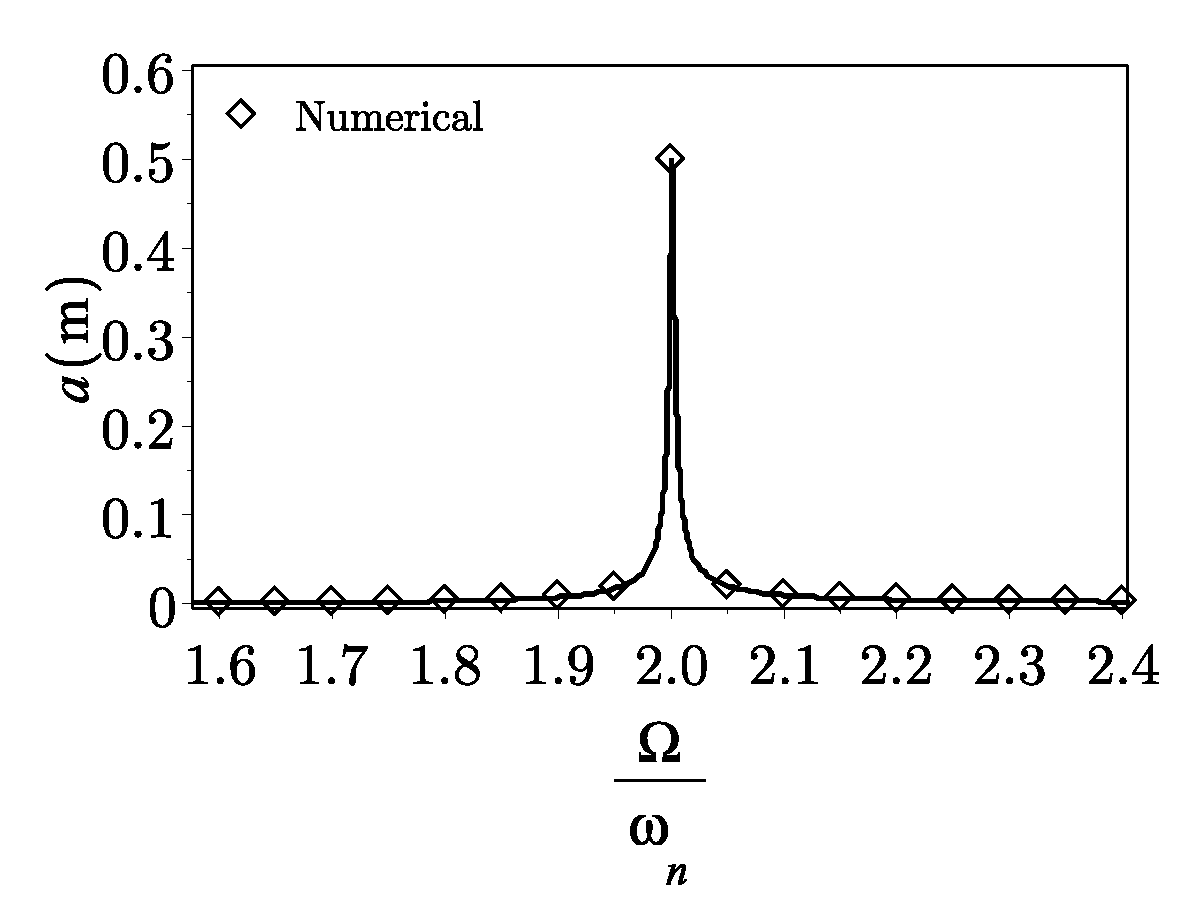
\includegraphics[width=0.8\textwidth]{Images/LinearCase.eps}}
\caption{Linear non-parametric}
\end{subfigure}
\qquad
\begin{subfigure}[b]{0.45\textwidth}
{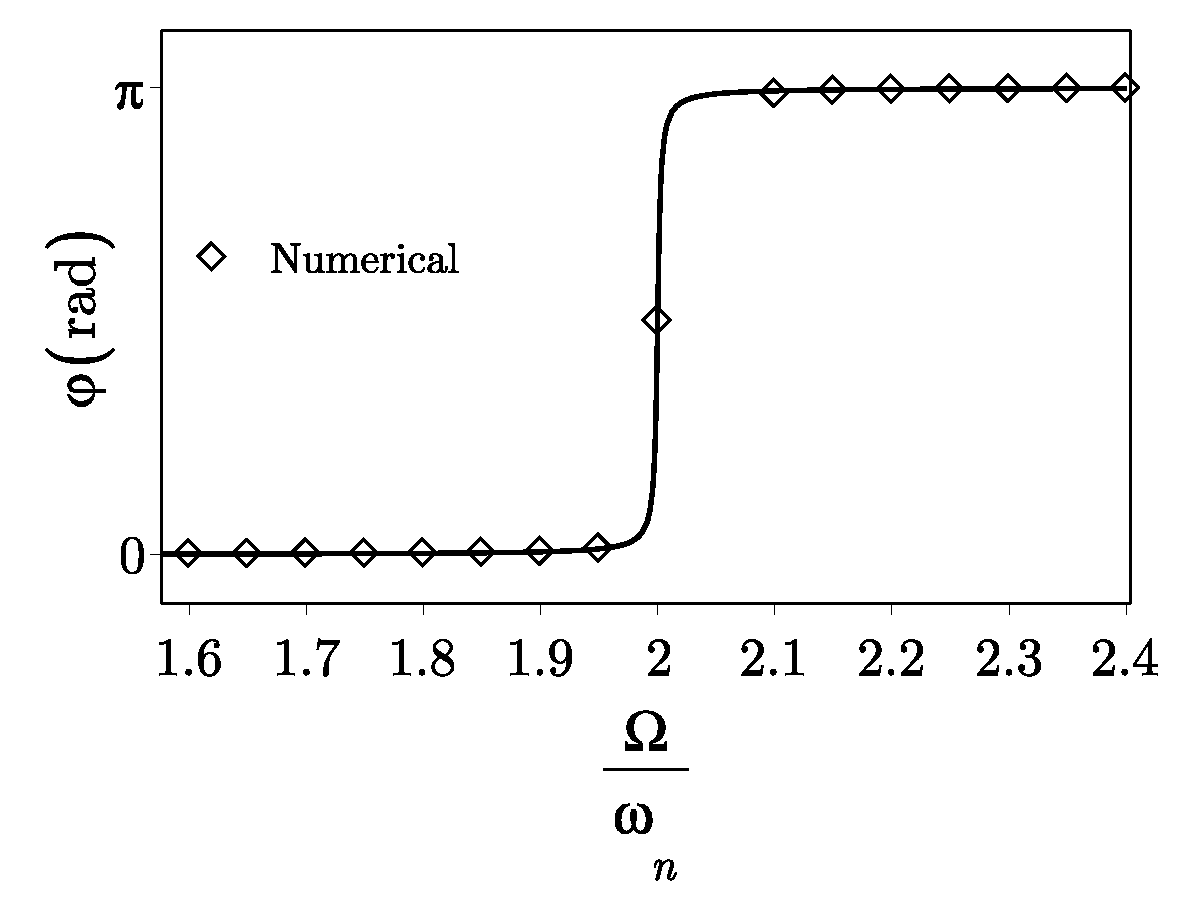
\includegraphics[width=0.8\textwidth]{Images/CaseAphaseFreq.eps}}
\caption{Linear non-parametric}
\end{subfigure}

\begin{subfigure}[b]{0.45\textwidth}
{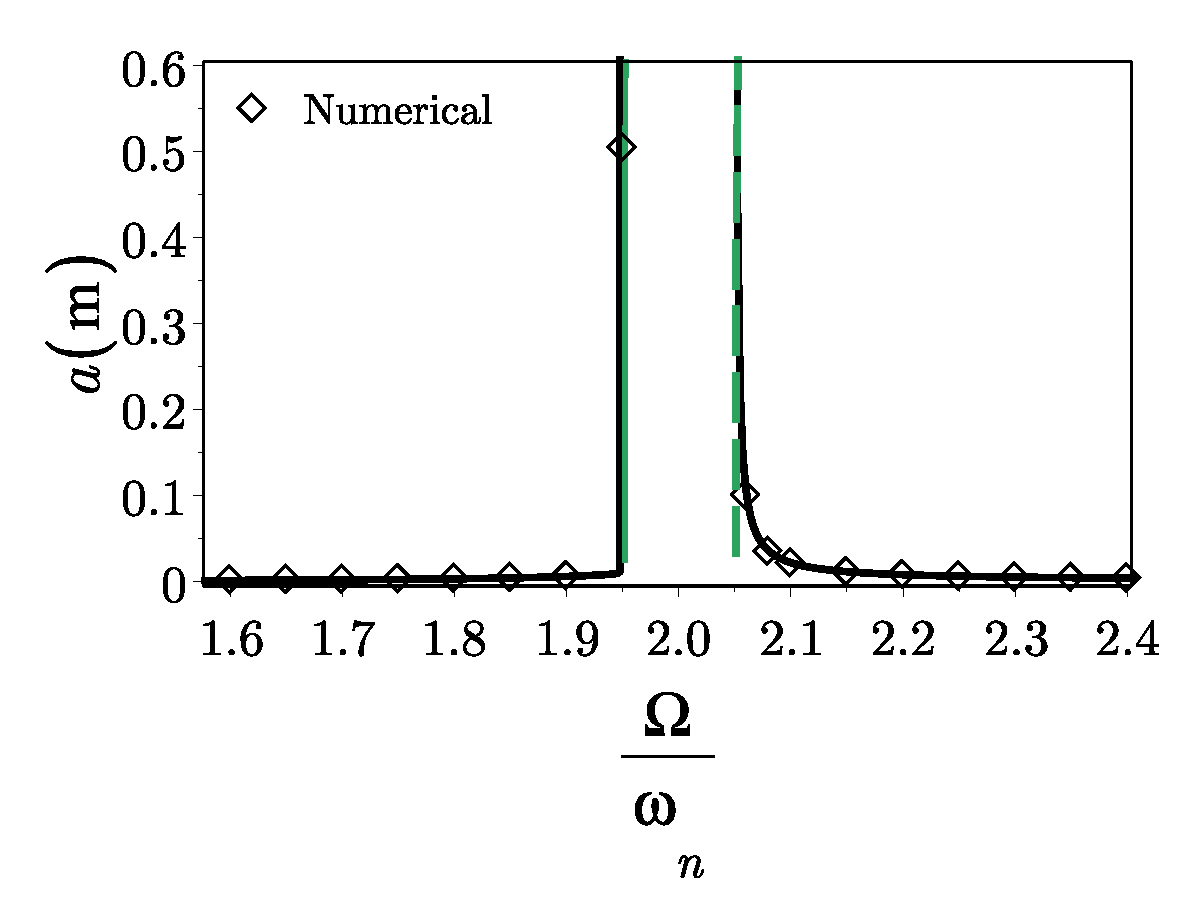
\includegraphics[width=0.8\textwidth]{Images/LinearPECase.eps}}
\caption{Linear parametric, above the instability threshold}
\end{subfigure}
\qquad
\begin{subfigure}[b]{0.45\textwidth}
{\includegraphics[width=0.8\textwidth]{Images/CaseBphaseFreq.eps}}
\caption{Linear parametric, above the instability threshold}
\end{subfigure}
%\caption{(\href{https://eprints.soton.ac.uk/399582/}{B. Zaghari, 2016})}
\end{figure}
\end{frame}
%%%%%%%%%%%%%%%%%%%%%%%%%%%%%%%%%%%%%%%%%%%%%%%%%%%%%%%%%%%%%%%%%%%%%
\begin{frame}{The effects of phase difference}
The gain associated with the LPE system is
\begin{equation}
\mathrm{Gain} = \frac{a\mid_{\delta \neq 0}}{a \mid_{\delta = 0}}.
\label{eq:gain}
\end{equation}
This gain is calculated analytically from the amplitude of the steady-state response.

\begin{figure}
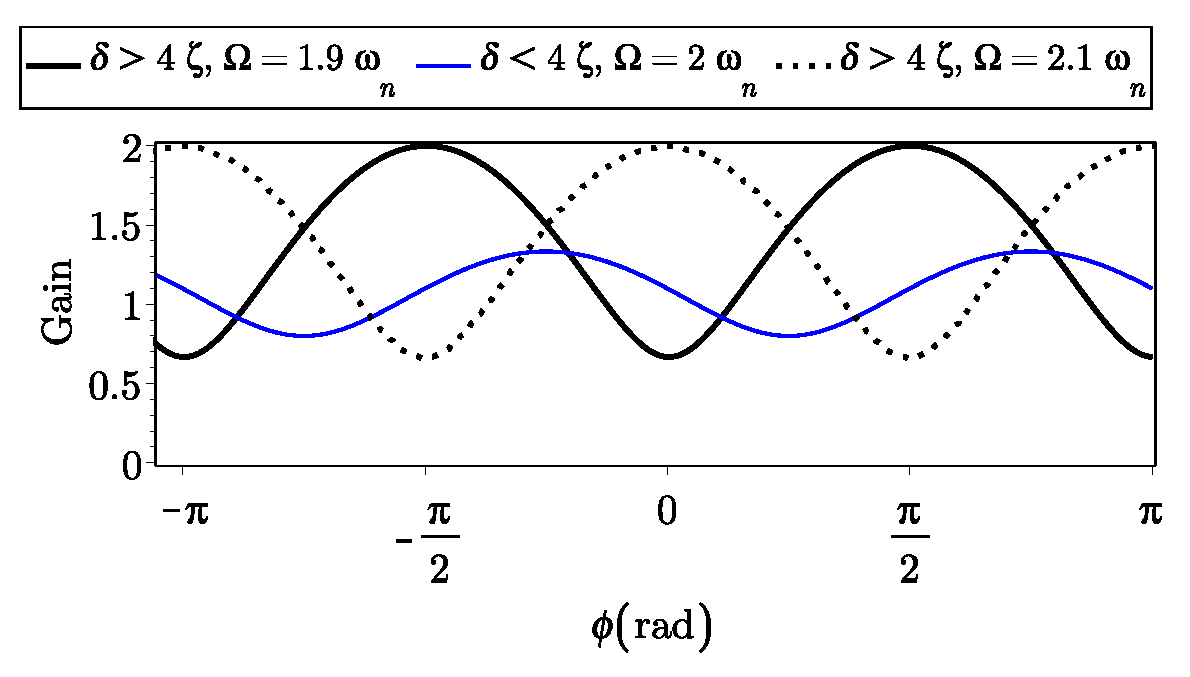
\includegraphics[width=0.7\linewidth]{Images/LinearPEPhase3Cases.eps}
\caption{Gain versus base excitation phase difference $\phi$ for a linear parametrically excited system (\href{https://eprints.soton.ac.uk/399582/}{B. Zaghari et al., 2016}).} 
\end{figure}
\end{frame}
%%%%%%%%%%%%%%%%%%%%%%%%%%%%%%%%%%%%%%%%%%%%%%%%%%%%%%%%%%%%%%%%%%%%%
\begin{frame}{The effects of time-varying damping}
\vskip-20pt
\begin{figure}
\begin{tabular}{*{2}{p{0.5\textwidth}}}
$c(t) = c_\mathrm{0} + c_\mathrm{p} \cos(\Omega t)$&\includegraphics[width=0.7\linewidth]{Images/SDOFC.eps}\\
&$x = X \cos(\omega t)$
\end{tabular}
\end{figure}
\begin{figure}
\textbf{Free vibration results, $x=0$}
\includegraphics[width=1.1\linewidth]{Images/displacement.png}
\caption{Relative displacement $z$ of the system for different values of parametric damping (a) $c_\mathrm{p} = -0.1 c_0$, (b) $c_\mathrm{p} = - c_0$, and (c) $c_\mathrm{p} = -4 c_0$ (\href{https://www.sciencedirect.com/science/article/pii/S0888327016000881}{M. Scapolan et al., 2017}).} 
\end{figure}
\end{frame}
%%%%%%%%%%%%%%%%%%%%%%%%%%%%%%%%%%%%%%%%%%%%%%%%%%%%%%%%%%%%%%%%%%%%%
\begin{frame}{The effects of time-varying damping - base excited case}
\begin{figure}
\includegraphics[width=0.75\linewidth]{Images/AveragePower.png}
\caption{Average harvested power for parametric damping close to instability and non-parametric damping. $\omega$ and $\omega_0$ are the base excitation and resonance frequency (\href{https://www.sciencedirect.com/science/article/pii/S0888327016000881}{M. Scapolan et al., 2017}).} 
\end{figure}
\end{frame}
%%%%%%%%%%%%%%%%%%%%%%%%%%%%%%%%%%%%%%%%%%%%%%%%%%%%%%%%%%%%%%%%%%%%%
\begin{frame}{Nonlinearity in parametrically excited systems}

\textbf{Why nonlinearity?}
\begin{itemize}
\setlength\itemsep{0.4cm}
	\item Real systems are nonlinear.
	\item Modern mechanical systems are more easily forced into a nonlinear regime.
\end{itemize}
\vspace{1em}
\textbf{Sources of nonlinearity:}
\begin{itemize}
\setlength\itemsep{0.4cm}
	\item Geometrical
	\item Material
	\item Nonlinear forces
	\item Physical configuration
\end{itemize}
\end{frame}
%%%%%%%%%%%%%%%%%%%%%%%%%%%%%%%%%%%%%%%%%%%%%%%%%%%%%%%%%%%%%%%%%%%%%
\begin{frame}{Electromagnetic system}
\begin{figure}
		\centering
		\includegraphics[width=\linewidth]{Images/5/CoilsSetup.eps}
		\caption{Electromagnetic forces generated by the current flow in coils are nonlinear forces and can influence the design of an electromagnetic energy harvester (\href{http://journals.sagepub.com/doi/full/10.1177/1077546318783566}{B. Zaghari et al., 2018}).}
	\end{figure}
\end{frame}	
%%%%%%%%%%%%%%%%%%%%%%%%%%%%%%%%%%%%%%%%%%%%%%%%%%%%%%%%%%%%%%%%%%%

\begin{frame}{Nonlinear parametrically excited (NPE) system}
%% Start tiks
\tikzstyle{na} = [baseline=-.5ex]

% Below we mix an ordinary equation with TikZ nodes. Note that we have to
% adjust the baseline of the nodes to get proper alignment with the rest of
% the equation.
\begin{equation*}
\ddot{z}+2 \varepsilon \zeta\omega_n\dot{z}+\omega_n^2\left(1+\varepsilon
        \tikz[baseline]{
            \node[fill=blue!20,anchor=base] (t1)
            {$\delta$};
        }\cos\left(\Omega t\right)\right)z + \omega_n^2 \left(\varepsilon
        \tikz[baseline]{
            \node[fill=red!20, ellipse,anchor=base] (t2)
            {$\alpha$};
        }+\varepsilon
        \tikz[baseline]{
            \node[fill=green!20,anchor=base] (t3)
            {$\gamma$};
        } \cos\left(\Omega t\right) \right) {z^3} = 0
\end{equation*}

\begin{itemize}[<+-| alert@+>]
    \item parametric amplitude 
        \tikz[na] \node[coordinate] (n1) {};
    \item cubic nonlinearity 
        \tikz[na]\node [coordinate] (n2) {};
    \item cubic parametric nonlinearity 
        \tikz[na]\node [coordinate] (n3) {};
\end{itemize}

% Now it's time to draw some edges between the global nodes. Note that we
% have to apply the 'overlay' style.
\begin{tikzpicture}[overlay]
        \path[->]<1-> (n1) edge [bend right] (t1);
        \path[->]<2-> (n2) edge [bend right] (t2);
        \path[->]<3-> (n3) edge [out=0, in=-90] (t3);
\end{tikzpicture}

\end{frame}
%%%%%%%%%%%%%%%%%%%%%%%%%%%%%%%%%%%%%%%%%%%%%%%%%%%%%%%%%%%%%%%%%%%
\begin{frame}{Nonlinear parametrically excited (NPE) system}
%% Start tiks
\tikzstyle{na} = [baseline=-.5ex]

% Below we mix an ordinary equation with TikZ nodes. Note that we have to
% adjust the baseline of the nodes to get proper alignment with the rest of
% the equation.
\begin{equation*}
\ddot{z}+2 \varepsilon \zeta\omega_n\dot{z}+\omega_n^2 \left(1+
        \tikz[baseline]{
            \node[fill=blue!5,anchor=base](t1)
            {$\varepsilon$};
        }\delta \cos(\Omega t)\right)z + \omega_n^2 \left(
        \tikz[baseline]{
            \node[fill=blue!5,anchor=base](t1)
            {$\varepsilon$};
        } \alpha + 
        \tikz[baseline]{
            \node[fill=blue!5,anchor=base](t1)
            {$\varepsilon$};
        } \gamma \cos(\Omega t) \right) {z^3} = 0
\end{equation*}

\begin{itemize}[<+-| alert@+>]
        \item bookkeeping parameter
        \tikz[na] \node[coordinate] (n1) {};
\end{itemize}

\begin{tikzpicture}[overlay]
        \path[->]<1-> (n1) edge [bend right] (t1);
\end{tikzpicture}

Stability and solutions of the nonlinear parametrically excited (NPE) system can be studied by:

\begin{itemize}
	\item The second method of Lyapunov 
	\item Methods of Harmonic Balance (HBM)
  \item Perturbation methods (Methods of Averaging, Multiple Scales, and Varying Amplitudes) 
\end{itemize}
\end{frame}
%%%%%%%%%%%%%%%%%%%%%%%%%%%%%%%%%%%%%%%%%%%%%%%%%%%%%%%%%%%%%%%%%%%%%%%%%%%%%%%%%%%%%%%%%%%%%%%%%%%%%%%%%%%
\begin{frame}{Effect of cubic stiffness nonlinearity}
\begin{figure}[h!]
		\centering
		\includegraphics[width=0.9\linewidth]{Images/4/AmplitudeFrequencyNonlinear1-0.eps}
		\caption{Analytical amplitude-frequency curves, \textcolor[rgb]{0,0,0}{$\varepsilon \alpha = 0.5 \mathrm{m^{-2}}$}, $\varepsilon \delta = 0.25$, $\varepsilon \zeta = 0.03$, and $\varepsilon \gamma = 0$.}
	\end{figure}
\end{frame}
%%%%%%%%%%%%%%%%%%%%%%%%%%%%%%%%%%%%%%%%%%%%%%%%%%%%%%%%%%%%%%%%%%%%%%%%%%%%%%%%%%%%%%%%%%%%%%%%%%%%%%%%%%%
\begin{frame}{Hardening nonlinearity}
	\begin{figure}[h!]
		\centering
		\includegraphics[width=0.9\linewidth]{Images/4/AmplitudeFrequencyNonlinear1-2.eps}
		\caption{Analytical amplitude-frequency curves, \colorbox[rgb]{1,0.28,0.28}{$\varepsilon \alpha = 150 \mathrm{m^{-2}}$}, $\varepsilon \delta = 0.25$, $\varepsilon \zeta = 0.03$, and $\varepsilon \gamma = 0$.}
	\end{figure}
\end{frame}
%%%%%%%%%%%%%%%%%%%%%%%%%%%%%%%%%%%%%%%%%%%%%%%%%%%%%%%%%%%%%%%%%%%%%%%%%%%%%%%%%%%%%%%%%%%%%%%%%%%%%%%%%%%
\begin{frame}{Softening nonlinearity}
	\begin{figure}[h!]
		\centering
		\includegraphics[width=0.9\linewidth]{Images/4/AmplitudeFrequencyNonlinear1-3.eps}
		\caption{Analytical amplitude-frequency curves, \colorbox[rgb]{1,0.41,0.13}{$\varepsilon \alpha = -150 \mathrm{m^{-2}}$}, $\varepsilon \delta = 0.25$, $\varepsilon \zeta = 0.03$, and $\varepsilon \gamma = 0$.}
	\end{figure}
\end{frame}
%%%%%%%%%%%%%%%%%%%%%%%%%%%%%%%%%%%%%%%%%%%%%%%%%%%%%%%%%%%%%%%%%%%%%%%%%%%%%%%%%%%%%%%%%%%%%%%%%%%%%%%%%%%
\begin{frame}{Frequency response plot for NPE}
	\begin{figure}[h!]
		\centering
		\includegraphics[width=\linewidth]{Images/4/NonlinEpsilonTransfer1-4.eps}
		\caption{$\varepsilon \zeta = 0.03$, $\omega_n = 31.62\mathrm{rad s^{-1}}$, $\varepsilon \delta = 0.25$, $\varepsilon \alpha = 150 \mathrm{m^{-2}}$, and $\varepsilon \gamma = 80 \mathrm{m^{-2}}$.}
	\end{figure}
\end{frame}
%%%%%%%%%%%%%%%%%%%%%%%%%%%%%%%%%%%%%%%%%%%%%%%%%%%%%%%%%%%%%%%%%%%%%%%%%%%%%%%%%%%%%%%%%%%%%%%%%%%%%%%%%%%
\begin{frame}{Frequency response plot for NPE}
	\begin{figure}[h!]
		\centering
		\includegraphics[width=\linewidth]{Images/4/NonlinEpsilonTransfer1-3.eps}
		\caption{$\varepsilon \zeta = 0.03$, $\omega_n = 31.62\mathrm{rad s^{-1}}$, $\varepsilon \delta = 0.25$, $\varepsilon \alpha = 150 \mathrm{m^{-2}}$, and $\varepsilon \gamma = 80 \mathrm{m^{-2}}$.}
	\end{figure}
\end{frame}
%%%%%%%%%%%%%%%%%%%%%%%%%%%%%%%%%%%%%%%%%%%%%%%%%%%%%%%%%%%%%%%%%%%%%%%%%%%%%%%%%%%%%%%%%%%%%%%%%%%%%%%%%%%
\begin{frame}
\begin{figure}
\begin{subfigure}[b]{0.35\textwidth}
{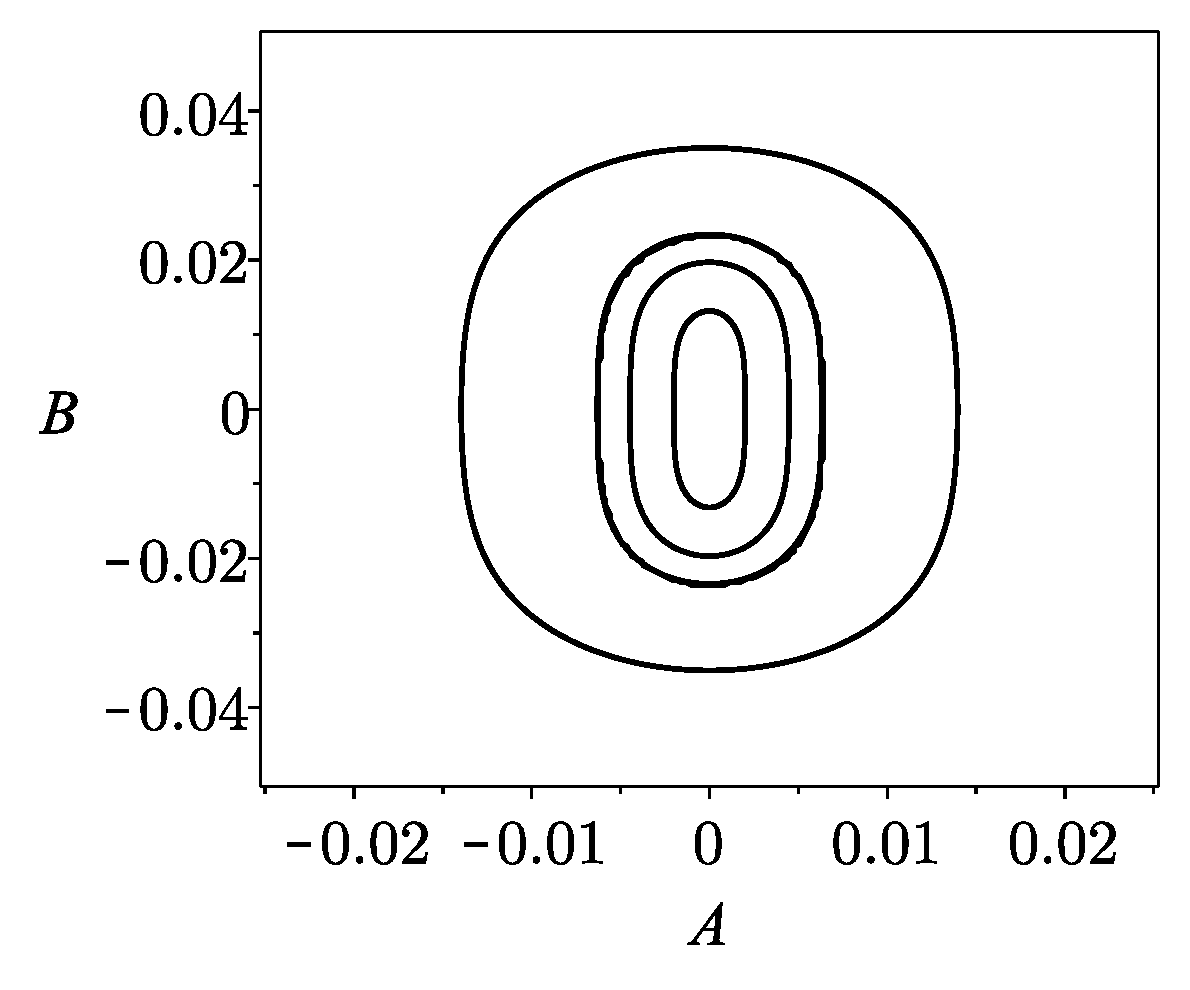
\includegraphics[width=\textwidth]{Images/PhasePortraitdeltaOver2.eps}}
\caption{}%\Delta=\frac{\delta}{2}
\label{fig:pointa}
\end{subfigure}%	
\begin{subfigure}[b]{0.35\textwidth}
{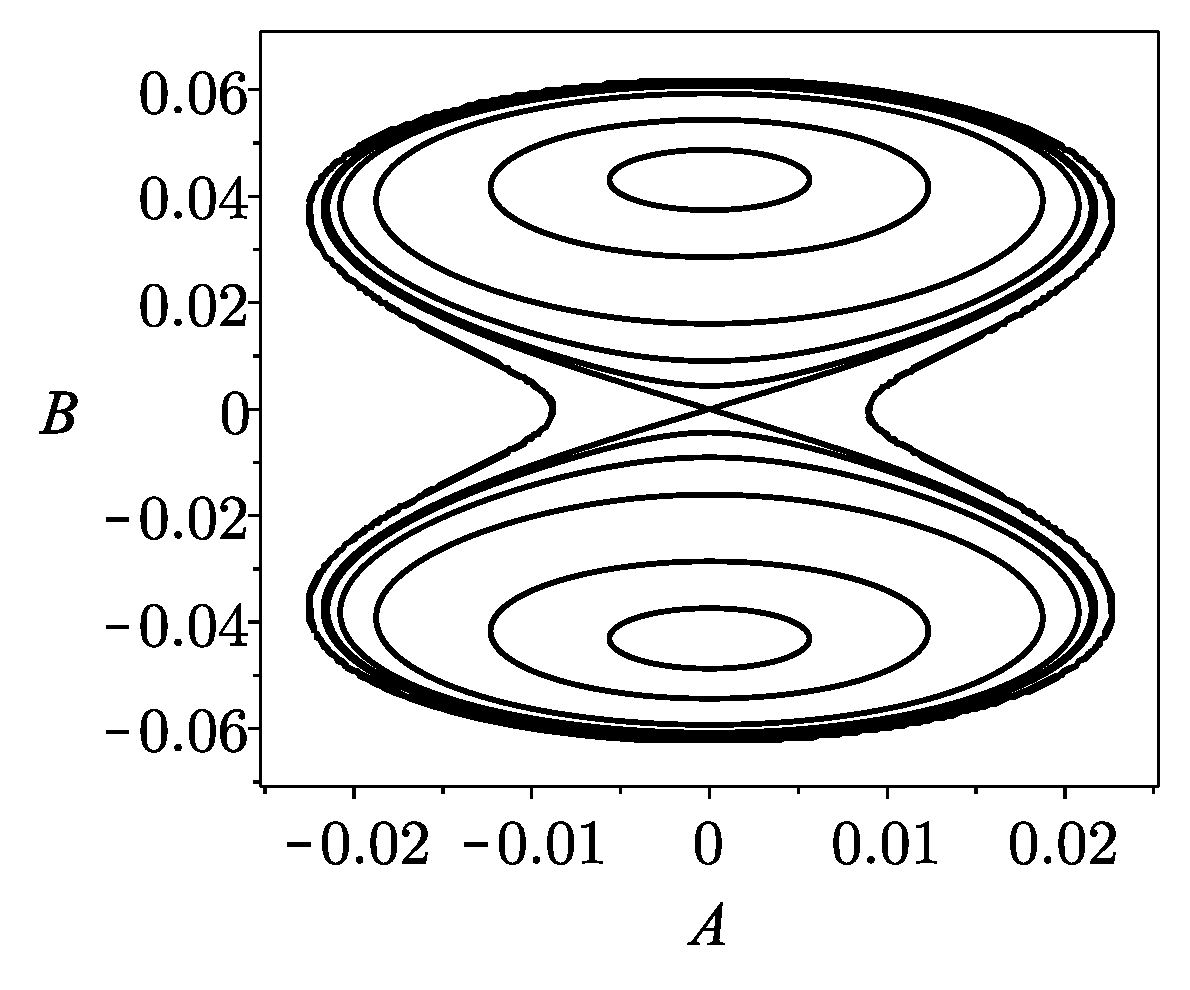
\includegraphics[width=\textwidth]{Images/PhasePortraitdeltaZero.eps}}
\caption{}%\Delta=0
\label{fig:pointb}
 \end{subfigure}%
\quad
\begin{subfigure}[b]{0.35\textwidth}
{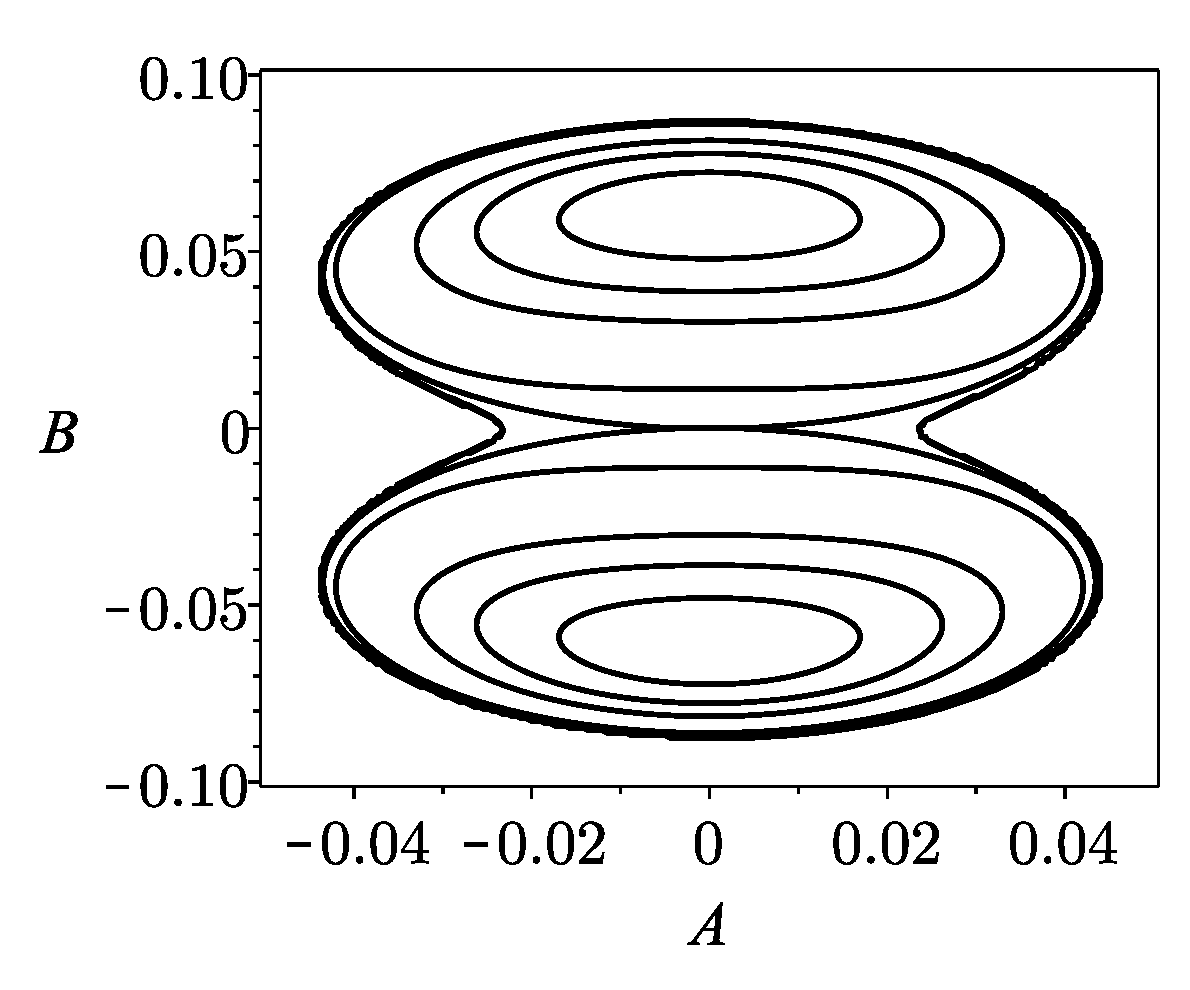
\includegraphics[width=\textwidth]{Images/PhasePortraitNdeltaOver2.eps}}
\caption{}%\Delta=-\frac{\delta}{2}
\label{fig:pointc}
\end{subfigure}%	
\begin{subfigure}[b]{0.35\textwidth}
{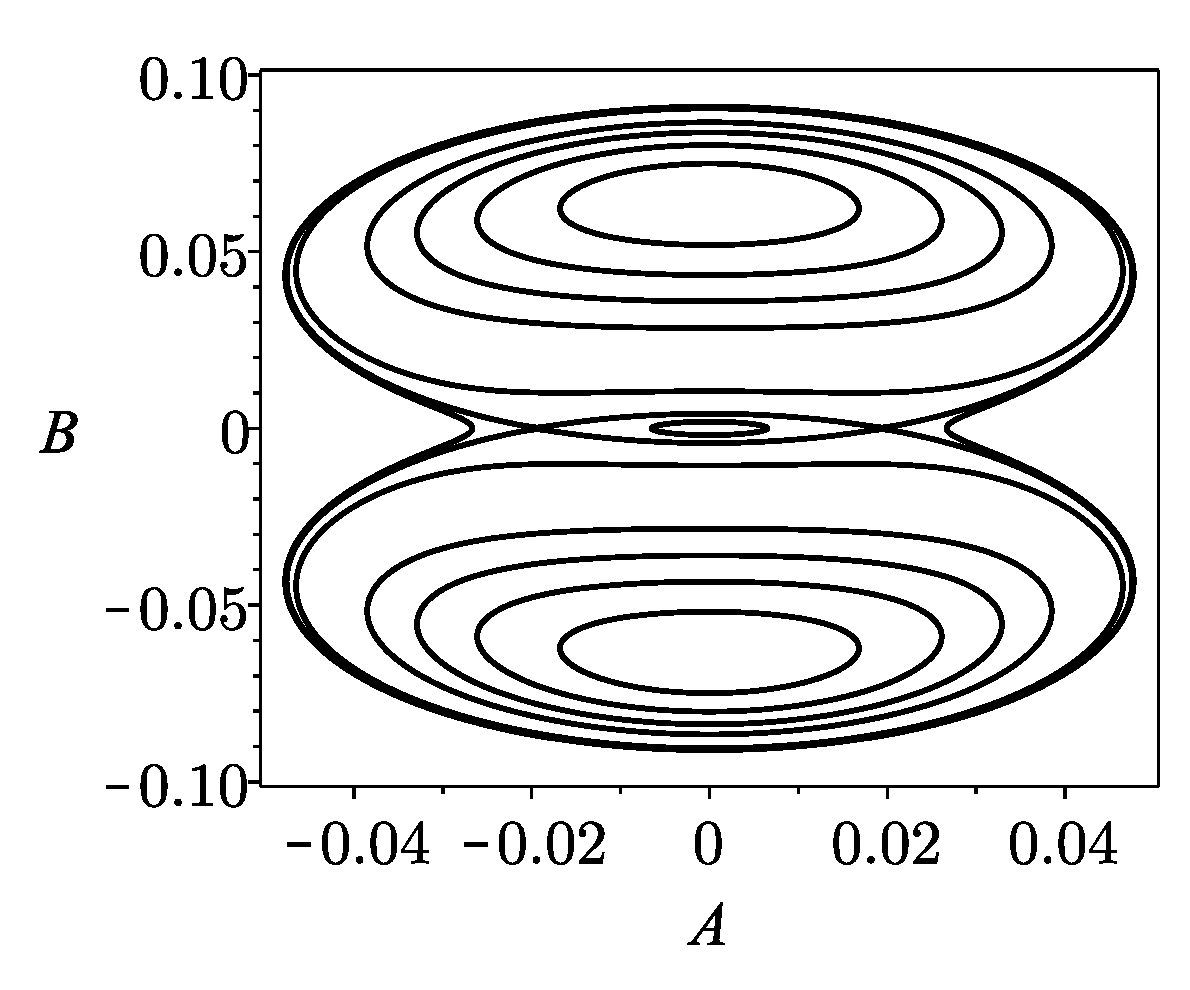
\includegraphics[width=\textwidth]{Images/PhasePortraitN1point2deltaOver2.eps}}
\caption{}%\Delta=-1.2\frac{\delta}{2}
\label{fig:pointd}
 \end{subfigure}%
\quad
\caption{The phase portraits correspond to different points on the transition curve when $\zeta=0$ (\href{https://eprints.soton.ac.uk/411397/}{B. Zaghari, 2016}).}
\label{fig:phasePortraitABplane}
\end{figure}
\end{frame}
%%%%%%%%%%%%%%%%%%%%%%%%%%%%%%%%%%%%%%%%%%%%%%%%%%%%%%%%%%%%%%%%%%%%%%%%%%%%%%%%%%%%%%%%%%%%%%%%%%%%%%%%%%%
\begin{frame}{Conclusions}
\begin{itemize}
\setlength\itemsep{0.75cm}
\item Vibration energy harvesting research is not mature yet. Many research challenges still exist in applying the technology.
\item The restrictions and limitations of real world environments must be continually designed around in order to create the best technology possible.
\item Linear harvesters produce more energy in most applications where a clear characteristic frequency is present.
\item Linear time-varying harvesters can increase the bandwidth and the power harvested.
\end{itemize} 
\end{frame}
%%%%%%%%%%%%%%%%%%%%%%%%%%%%%%%%%%%%%%%%%%%%%%%%%%%%%%%%%%%%%%%%%%%%%%%%%%%%%%%%%%%%%%%%%%%%%%%%%%%%%%%%%%%
\begin{frame}{Acknowledgement}
\centering \Large
Funding from EPSRC Platform Grant, Clean Sky, and EnABLES.
\\~\\~\\ \small
I would like to thank Prof. Steve Beeby, Prof. Neil White, Prof. Ling Wang, Dr. Alex Weddell, Dr. Emiliano Rustighi, Dr. Maryam Ghandchi Tehrani, Dr. Fadi Dohnal, and Prof. Subhash Sinha.
\\~\\~\\
\emph{Thank you}\\[2em]These slides are available on GitHub at https://tinyurl.com/y9uwtz3q.
\end{frame}
%%%%%%%%%%%%%%%%%%%%%%%%%%%%%%%%%%%%%%%%%%%%%%%%%%%%%%%%%%%%%%%%%%%%%%%%%%%%%%%%%%%%%%%%%%%%%%%%%%%%%%%%%%%
\end{document} 